\documentclass[]{article}

\usepackage[style=ieee,backend=bibtex]{biblatex}
\PassOptionsToPackage{margin=1in}{geometry}
\usepackage{wordlike}
\usepackage{setspace}
\usepackage{parskip}
\usepackage{graphicx}
\usepackage{listings}

\setstretch{1.5}


%opening
\title{How Open is Open Source? Metrics for measuring software mutation}
\author{Charles Hathaway}

\bibliography{biblo}

\begin{document}

\maketitle

\begin{abstract}

Open source software is toted as being "openly accessible" to many people, thus allowing greater innovation and complex new methodologies.
However, given the complexity of software and how difficult it is to design and implement, the question of whether or not secondary communities adapt and modify the software needs to be addressed.
This paper poses the question of determining the involvement of multiple communities to a project by measuring their contributions in terms of complexity, and discusses how we would go about measuring contributions to a project in a meaningful way.

\end{abstract}

\section{Introduction}

% What is open source? very brief regurgitation
% Why do we care about open source? list large projects that "matter"
% --> Include projects listed as "can not fail" internet services
% Does it matter how open projects are?
% How will being able to measure how open projects are help organize things

Open Source software, which includes such well known projects as Linux, Apache, and OpenSSL, has a large portion of todays market share in their respective segments.
According to reports available from w3techs \cite{w3techs2015usage}, *nix systems account for 67.7\% of the internet web servers; 52.7\% of these are running a Linux distribution. 
Important projects, such as OpenSSL, attract world-wide media attention when severe bugs appear; take for example the numerous articles published because of the April 2014 bug called "Heartbleed" \cite{mitre2013heartbleed}  \cite{whittaker2014heartbleed}.

After this particular crisis, it was realized that there are numerous open source projects that are too big to fail.
Large corporations agreed to contribute money to these projects, in hopes that it will prevent another such bug \cite{brodkin2014heartbleed}.
It is here where we can begin to understand the need to figure out who is working on projects, how much are they doing, and how complicated the projects are.

Understanding who is working on a project is no simple matter; we must consider multiple roles (programmer, tester, project manager, to name a few), along with the amount of work they are putting into that project (are they spending 1/8 of their day on it? 16/24 of their day?).
This paper, will propose a method for further research that will allow one to quantify the contributions of at least one role in a software developers world; the role of the programmer.
Namely, what we want to discover is how we can measure the change that a developer causes in the codebase; are they simply renaming variables, adding UI elements, or changing core algorithms?
This question of the distribution of coding contributions might have several applications: for example knowing the degree to which modified code has changes in complexity arises in assessment of students' work in education; in the assessment of originality in legal domains; and even the assessment of  biological material if we think of genetics or amino acid sequences as code.

This brings us into the field of software complexity.
It is important not to confuse this field with other forms of complexity we often look at in the computer science discipline, such as time and space complexity.
The goal of this field is to determine how difficult a program is to understand, test, and write.

There have been many attempts over the years to measure software complexity; some of the most well known ones by McCabe \cite{ref:a_complexity_measure}, Oviedo \cite{ref:oviedo1993control}, and Halstead \cite{ref:halstead1977elements}.
Our goal in this paper is to develop a method which can eventually be used to evaluate the most common complexity measures, and look for correlations between how real people percieve a program to be, and how the metrics understand the complexity of a program.
To conclude the paper, we will run a small-scale experiment on 5 people, asking them to rank 5 projects (which produce similar output) on how complex they appear to be.
Later research will repeat this experiment on a larger, and more diverse, group of subjects.

For simplicity, this paper will utilize the visual programming environment created for the 3Helix program at Rensselaer Polytechnic Institute, CSnap.
These scripts are best stored (for long term access) as images, and will be included at the end of the paper.

\section{Literature Review}

% We have at least 2 distinct "areas" to review; open source-ness, and ways of measuring software similiarity

As a form of literature review, will use a subset of well-known papers that represent some of the most important works in this field.
Most of these articles have been reprinted \textbf{Software Engineering Metrics Volume 1} \cite{sheppherd1993complexity}, including:
\begin{itemize}
	\item \textbf{A Complexity Measure} \cite{ref:a_complexity_measure}
	\item \textbf{Control Flow, Data Flow, and Program Complexity} \cite{ref:oviedo1993control}
\end{itemize}

It is worth mentioning that most of these metrics have had their accuracy questioned, and for the most part been proven to fail in one or more ways.
A very well known paper that described the failure of these metrics is \textbf{Evaluating Software Complexity Measures}, written in 1988 by Elaine J. Weyuker \cite{ref:evaluating_software_complexity_measures}.
Weyuker's has been used as the core for many following software complexity papers, including the recent publication by Hongwei Tao, \textbf{Complexity measure based on program slicing and its validation} \cite{ref:tao2014complexity}.


% More stuff?

\subsection{Evaluating Software Complexity Measures}

% We need to talk about everything, including silly things like...
% Lines of code changed

In this section, we will summarize and describe previous metrics, with particular attention to Weyuker's analysis.
For convenience, I have copied the 9 properties of complexity measures she proposed here. 
Note, however, that they are explained in greater detail in the paper.

In the following statements, P and Q represent entire programs.
In order to satisfy each property, the metric result of each of the proposed methods must satisfy all of these properties to be considered correct; the use of carnality operators in the context returns the result of a particular metric algorithm instead of the length of a program.
% begin comment msk -
%You have to explain what P and Q are Are they Programs/Predicates -
%Intuition behind each of these properties have to be esplained
% end comment msk

\begin{itemize}
	\item Property 1: $(\exists P)(\exists Q)(|P|\neq |Q|)$
	\begin{itemize}
		\item There exists a program P and a program Q such that the complexity of program P does not equal the complexity of program Q. ie, not all programs have the same complexity
	\end{itemize}
	\item Property 2: Let c be a nonnegative number. Then there
are only finitely many programs of complexity c.
	\begin{itemize}
		\item There is a limit to the number of programs at complexity c
	\end{itemize}
	\item Property 3: There are distinct programs P and Q such
that $|P| ~= ~|Q|$
	\begin{itemize}
		\item There are two programs that do have the same complexity measure
	\end{itemize}
	\item Property 4: $(\exists P)(\exists Q)(P \equiv Q ~\& ~|P| \neq |Q|)$
	\begin{itemize}
		\item Programs P and Q produce the same output, but don't have the same complexity
	\end{itemize}
	\item Property 5: $(\forall P)(\forall Q)(|P| \leq |P; Q| ~and ~|Q| \leq |P; Q|)$
	\begin{itemize}
		\item In all cases, adding together programs doesn't make them less complex
	\end{itemize}
	\item Property 6a: $(\exists P)(\exists Q)(\exists R)(|P| = |Q| \& |P;R| \neq |Q; R|)$
	\item Property 6b: $(\exists P)(\exists Q)(\exists R)(|P| = |Q| \& |R;P| \neq |R; Q|)$
	\begin{itemize}
		\item Taken together, 6a and 6b are meant to say that adding the same program to existing programs, with the same complexity, doesn't necessarily mean that the two programs will still have the same complexity; for example, variables may interact in such a way as to make it much more complicated.
	\end{itemize}
	\item Property 7: There are program bodies P and Q such that Q is formed by permuting the order of the statements of P, and $|P| \neq |Q|$
	\begin{itemize}
		\item The order of the statements has an impact on complexity; ie, the same statements in a different order can mean something more complicated
	\end{itemize}
	\item Property 8: If P is a renaming of Q, then $|P| = |Q|$
	\begin{itemize}
		\item Simply changing the name of our variables shouldn't impact the complexity of the program
	\end{itemize}
	\item Property 9: $(\exists P)(\exists Q)(|P|+|Q| < |P; Q|)$
	\begin{itemize}
		\item Adding the complexity of two programs could result a complexity number lower than adding the two programs together and taking the complexity again
	\end{itemize}
\end{itemize}

\subsection{Summarization of Control Graphs}

Control graphs are used by many metrics, and rather than repeating their design in every section, I will describe them here. 
There has been some change in the nature of computer programming which makes many of the graphs demonstrated in older literature obsolete, namely the case where a GOTO drops execution into a loop or conditional from elsewhere.
We will set aside this case, to make the generation much more simple.

Given a program start point, P, add every statement to a node N until a conditional (or loop) node is reached.
At this point, create a new node to represent the conditional, and follow all new paths.
When they end, join them into a new node.
If we are dealing with a loop, when we reach the end of the loops inner block, draw a line back to our loop node. 
Then connect the loop node to a new node. 
To help clarify, some sample programs, (along with their graphs) are given below.



\subsection{Cyclomatic complexity}

Thomas McCabe proposed a complexity measure in his 1976 paper \cite{ref:a_complexity_measure}.
In this section, I will briefly describe how it works, how to calculate it, and discuss some responses to it (specifically the responses made by  Elaine Weyuker in her 1988 paper \cite{ref:evaluating_software_complexity_measures}).

\subsubsection{How it works}

The McCabe metric (Cyclomatic number) analyses the control flow of a program to determine how complex it is. 
There are 3 primary items that is used the calculation of the cyclomatic number:
\begin{itemize}
	\item Number of nodes, denoted as n
	\item Number of edges, denoted as e
	\item Number of compontents, denoted as p
\end{itemize}

Given these three variables, we can calculate a complexity ($\mu$) of a program using the following equation:

$\mu ~= ~e ~- ~n ~+ 2p$

It should be noted that we use 2p instead of p; some books use p, but draw an exra edge back to the start node from the end node in each component.
These two methods result in identical complexities, but I prefer the second because it makes it easier to identify the start and end nodes in my program.

The real challenge is to create the graph so you can find values for these variables.
To do this you must break a program into parts such that there is a starting node, and ending node, and a sequence of nodes between that two have the following key attributes:
\begin{itemize}
	\item A compound statement is only one node; ie, int i=0; i = b*x; ... counts as only one node until the next branch occurs
	\item A branch is a conditional, either in the form of an if statement or a loop (with a loop, connect the node to both the following statement(s) and the code that gets executed after it exits)
\end{itemize}

As a general rule of a thumb, we have a component anywhere a loop occurs.
We can have multiple components inside a component (embedded loops). 

Once we have created a graph, it is a trivial matter of counting the number of edges, nodes, and components and applying the equation.

\subsubsection{Example}

Looking at the control graph for the first program, see figure \ref{alpha}, we can calculate the cyclomatic number pretty easily.
There are 2 edges, 3 nodes, and 1 component.
Therefore, our cyclomatic number is:

$\mu ~= ~e ~- ~n ~+ 2p ~= ~2 ~- ~3 ~+ 2(1) ~= 1$

In this figure, we can see that all statements get put into one node.
More complicated graph, such as the one for program delta in figure \ref{delta}, allow to see how the control flow graph is generated more intuitively.

\subsubsection{Analysis}

This metric was included in the analysis performed by Weyuker in her 1988 paper \cite{ref:evaluating_software_complexity_measures}.
Ultimately, she concluded that McCabes metric failed to address properties 2, 6, 7, and 9, for the following reasons:
\begin{itemize}
	\item Property 2: We can easily imagine an infinite number of programs that don't branch, but are just repeats of the same statement over and over (x+=2;x+=2;x+=2..). These programs would have a complexity of 1, and there are an infinite number of them
	\item Property 6: Since McCabes complexity measure doesn't account for the interaction of variables, appending a program (R) to the end of another program (P) would always result in $|P|+|R|$, whichs means that if $|Q|=|P|$, then $|Q|+|R| ~= ~|P|+|R|$.
	\item Property 7: The order of statements in McCabe's metric have no influence on complexity; we will always have the same number of branches, same number of nodes, and components
	\item Property 9: McCabe's metric fails this for the same reason as property 6
\end{itemize}

Additional critique was made by Martin J. Shepperd in his 1988 paper \cite{shepperd1988critique}, however we found some discrepancies between this critique and the model developed by McCabe.

\subsection{Normalized Compression Distance}

Proposed by Rudi Cilibrasi and Paul Vitanyi in their 2005 paper, \textbf{Clustering by compression} \cite{ref:cilibrasi2005clustering} puts forth a very straightforward way of calculating complexity changes between two pieces of code, without even knowledge of the structure of the content.
They envisioned this method being used to cluster data for machine learning, however, we believe it may also be a good way to measure change between two programs; if the distance between a start point and an end point are large, there was a great deal of change.
If the distance is not significant, there was not a significant amount of change.
They proposed using a standard compression method (such as gzip or PPMZ) to approximate the Kolmogorov complexity of a program, and using this solve the equation in figure \ref{ncd_eq_1}.


\begin{figure}[h]
	\caption{Normalized Compression Distance}
	\label{ncd_eq_1}
	\centering
	$NCD(x,y) ~= \frac{C(xy) - min(C(x),C(y))}{max(C(x),C(y))}$
\end{figure}

There is some additional difficulty involved in computing this from CSnap projects; a large portion of the XML file is simply constant data, such as the program version, stage size, etc.
Therefore, to make this more accurate, we only compress and compare the script sections of the XML file.
This still isn't perfect, since XML has so much additional data, but it a better approximation than using an entire file.

\subsubsection{Example}

If we attempt to compare projects alpha and beta, we can get the NCD by extracting the scripts, compressing them, and performing the outlined calculation listed above.
The raw XML code is too long to insert here, however, it can be obtained from the data repository in the files "sample\_csnap\_applications/alpha\_script.xml" and "sample\_csnap\_applications/beta\_script.xml".

If we compress these files using gzip, the record the sizes of the new files, we can do the calculation.

\begin{lstlisting}
[charles@aura sample_csnap_applications]$ cp alpha_script.xml alpha_beta_script.xml
[charles@aura sample_csnap_applications]$ cat beta_script.xml >> alpha_beta_script.xml
[charles@aura sample_csnap_applications]$ ls *_script.xml
alpha_beta_script.xml  alpha_script.xml  beta_script.xml
[charles@aura sample_csnap_applications]$ gzip *_script.xml
[charles@aura sample_csnap_applications]$ ls -l *_script.xml.gz
-rw-rw-r--. 1 charles charles 380 May  7 14:41 alpha_beta_script.xml.gz
-rw-rw-r--. 1 charles charles 278 May  7 14:37 alpha_script.xml.gz
-rw-rw-r--. 1 charles charles 315 May  7 14:37 beta_script.xml.gz

\end{lstlisting}

With our variables not set to:

\begin{itemize}
	\item $C(x) ~= ~278$
	\item $C(y) ~= ~315$
	\item $C(xy) ~= ~380$
\end{itemize}

We can use the equation to calculate NCD:

$NCD(x,y) ~= \frac{C(xy) - min(C(x),C(y))}{max(C(x),C(y))}$

$NCD(x,y) ~= \frac{380 - min(278,315)}{max(278,315)}$

$NCD(x,y) ~= \frac{380 - 278}{315}$

$NCD(x,y) ~= ~0.3238095238095238$

\subsubsection{Analysis}

Weyuker did not analyze this metric in her paper, and as of the time of writing this paper, no one has attempted that comparison.
This is may be due to the fact that we don't normally analyze the distance between two sets of code as a metric, even though many of Weyukers metrics are entirely about finding a change between two pieces of code.

In this section, we compare primarily programs P and Q.
Rather than do something funky with comparing them to each other, we can imagine reducing NCD with an input of NCD(x,x), which can be reduced as demonstrated in figure \ref{ncd_reduction}.

\begin{figure}[h]
	\caption{Normalized Compression Distance Reduction}
	\label{ncd_reduction}
	\centering
	$NCD(x,x) ~= \frac{C(xx) - min(C(x),C(x))}{max(C(x),C(x))}$
	$NCD(x,x) ~= \frac{C(xx) - C(x)}{C(x)}$
	$NCD(x,x) ~= \frac{C(xx)}{C(x)} ~- ~\frac{C(x)}{C(x)}$
\end{figure}


Rather than just end there though, let's discuss a few things.
First, Normalized Compression Distance relies on a normal compressor, as discussed in Cilibrasi's paper \cite{ref:cilibrasi2005clustering}.
It has the following attributes:
\begin{enumerate}
	\item Idempotency: C(xx) = C(x).
	\item Monotonicity: C(xy) ≥ C(x).
	\item Symmetry: C(xy) = C(yx).
	\item Distributivity: C(xy) + C(z) ≤ C(xz) + C(yz).
\end{enumerate}

Which means we can further reduce this to further, to eventually, 1.
Does this mean that all programs should have a NCD metric of 1, if compared to themselves?
My assertion, for the purpose of doing this evaluation, is that they should not.

What if we use a program, y, which has a size of 0.
In this case, we still end up with C(x)/C(x), which is 1.
So we can't do that.

What if, instead, we had a program y, which is the same length of x, such that there is no way to get C(xy) that does not equal C(x)+C(y)?
This provides us with a much better way to analyze the sitation; 

% % This doesn't work.

We provide a brief pass over all of Weyuker's properties with NCD in mind, and give an explanation as to why each is or isn't satisfied. 
We will not do rigid proofs, but rather leave those for an area of later research.

\begin{itemize}
	\item Property 1: $(\exists P)(\exists Q)(|P|\neq |Q|)$
	\begin{itemize}
		\item This can easily be demonstrated; just look at the example we give in the appendix. There are 4 programs, all of which have different complexity ratings.
	\end{itemize}
	\item Property 2: Let c be a nonnegative number. Then there
are only finitely many programs of complexity c.
	\begin{itemize}
		\item Given that for NCD a program is just a compression of source code, we could expect a program with contents 'x+=1;' to smaller than a program with contents 'x+=1;y+=1'.
	\end{itemize}
	\item Property 3: There are distinct programs P and Q such
that $|P| ~= ~|Q|$
	\begin{itemize}
		\item This is harder to envision, but if we had two programs that were the same code moved around, then compressed, we would get the same complexity size. Take a program (in some hypothetical language) that consisted of the code "x+=1;y+=1", and it's brother program that consisted of "y+=1;x+=1". Compressing these programs results in a NCD metric of 34 for both
	\end{itemize}
	\item Property 4: $(\exists P)(\exists Q)(P \equiv Q ~\& ~|P| \neq |Q|)$
	\begin{itemize}
		\item As long as the two programs aren't identical, and aren't permutations of each other, we could imagine two programs with different NCD's and the same output
	\end{itemize}
	\item Property 5: $(\forall P)(\forall Q)(|P| \leq |P; Q| ~and ~|Q| \leq |P; Q|)$
	\begin{itemize}
		\item Although in our examples it *may* be possible to prove this one wrong, this is most likely due to our not-quite-perfect compression; one could imagine that with a perfect compression, you could get a metric that is the same size, but not smaller \footnote{Note that we are ignoring cases where two operations, when taken together, can be simplified to a single (or no) operation; our goal is to evaluate program complexity, not whether or not is optimal.}
	\end{itemize}
	\item Property 6a: $(\exists P)(\exists Q)(\exists R)(|P| = |Q| \& |P;R| \neq |Q; R|)$
	\item Property 6b: $(\exists P)(\exists Q)(\exists R)(|P| = |Q| \& |R;P| \neq |R; Q|)$
	\begin{itemize}
		\item NCD will account for this; if program R has subsets of program Q in it, it would result in a different size than program R;Q
	\end{itemize}
	\item Property 7: There are program bodies P and Q such that Q is formed by permuting the order of the statements of P, and $|P| \neq |Q|$
	\begin{itemize}
		\item This can be proven by taking the beta\_script.xml and moving the clear block; the resulting file has a larger size than the original
	\end{itemize}
	\item Property 8: If P is a renaming of Q, then $|P| = |Q|$
	\begin{itemize}
		\item NCD would fail in this respect; longer variable names would result in longer compressed scripts
	\end{itemize}
	\item Property 9: $(\exists P)(\exists Q)(|P|+|Q| < |P; Q|)$
	\begin{itemize}
		\item It is unlikely this would be true for NCD; adding two programs together gives the compressor more to work with, and therefore it would be able to do a better job. Just adding the size of the smaller compressed files would fail to work (just think about the overhead we have to add in! Program "ab" went from size 3 to size 29 when we compressed it).
	\end{itemize}
\end{itemize}

% % TODO! More

%\subsection{Effort measure}
% Forgo this section for now, I'm missing the book where it is defined
% Need to trace this back I think
% This is sort of the thing that Ron's expirement would look at
%\cite{ref:evaluating_software_complexity_measures}

\subsection{Data flow complexity}

Enrique Oviedo proposed a metric based on data flow in his 1980 paper \cite{ref:oviedo1993control}.
This metric is based on 2 key components; data flow (DF) and control flow (CF).
He concludes with the equation $C = \alpha CF + \beta DF$ (where $\alpha=\beta=1$).
% This later followed up be ... who said \alpha should equal and \beta should equal...

%begin comment msk
% You need to give an example here - The notations are not known in the compiler area 
%end comment msk

\subsubsection{How it works}

Control flow is simply the cardinality of the program flow graph.
The program flow graph, and how to construct it, is clearly defined in the paper.
It more or less follows the same structure as the graphs we construct for the Cyclomatic number, with a more formal definition being given to how a "program" (function in modern terminology) is denoted.
Formally,

$CF=\parallel E\parallel$

Where $\parallel ~\parallel$ stands for set cardinality.

The more complicated part of this metric is the data flow measure.
The key terminology for this measure is the distinction between a locally available variable and a locally exposed variable.
A variable is locally available when the variable is defined in the block (a block is a "node" in our control flow).
A variable is locally exposed when it is referenced without being defined in the block.
Another important note is that a variable can be "overridden" (killed) in a block if it is locally exposed, and then made locally available.

$DF_i = \sum\limits_{j=1}^{\parallel V_i \parallel} DEF(v_j)$

Where $V_i$ is the set of exposed variables in this block and $DEF(v_j)$ counts the number of available definitions for $v_j$; that is, for j from 1 to length(the set of variables that reach block i) add the number of definitions of variable j to the running total.
The example given by Oviedo is:
\begin{quotation}
	For example, if block $n_i$ consists of the statements \textit{X = Y; A = B * Y * ( C - B ); Z = 2 + A;} and the set of variables definitions that can reach block $n_i$ is $R_i ~= ~{C_j, B_j, Y_k, B_k}$ (ie, if the definitions of C and B in block $n_j$ and the definitions of Y and B in block $n_k$ can reach block $n_j$), then, according to Definition 8, we have $V_i ~= ~{C,B,Y}$ and
	
	$DF_j = \sum\limits_{j=1}^{3} DEF(v_j)~=~4$ \cite{ref:oviedo1993control}
\end{quotation}

Although some authors (for example, the author of the very well known Principles of Compiler Design \cite{aho1977principles}) utilize DEF alongside other functions, such as KILL and USE, these are not described in Oviedo's paper.

$DF = \sum\limits_{i=1}^{\parallel S \parallel} DF_i+DF_f$

Where S is all nodes except the start and the end nodes.

%begin comment msk
%you have to give example numbers for one of the examples and explain 
%end msk

\subsubsection{Analysis}

This metric was included in the analysis performed by Weyuker in her 1988 paper \cite{ref:evaluating_software_complexity_measures}.
Ultimately, she concluded that the Dataflow metric failed to address properties 2 and 5.

\subsection{Other metrics}

In addition to the above stated metrics, we will also consider lines of code (also referred to as statement count).
This metric is almost universally accepted as not indicative of the complexity of a program, and will provide a sane reference point to verify that we are not just finding correct data.

Lines of code is very dependent on the language in which we are evaluating programs.
Since we are using CSnap as a small-scale staging run, we will consider a "line of code" to be a command block (as defined by Snap! and CSnap).
These blocks include things such as "if", "go to {x coordinate}", etc.

\section{Measuring change}

% We really need to decide what to do about this :(

% Propose new metric in this paper and test with the toy example (small)

% Most likely an aggregate metric, but what weights and metrics?

There are several issues that need to be addressed by our algorithm of we are to effectively measure change in software over a large period of time.
These include:
\begin{itemize}
	\item Accounting for "non-changes"; ie, making a change to a project, testing it, then changing it back
	\item Discerning between changes that required little to no effort, and changes that may only have been to a line or two, but required a great deal of effort
	\item Considering things that change the output as part of the metric; not all changes will change the end-result of a program, but will rather optimize the process; other changes will cause the behavior of the program to dramatically alter. How do we differentiate these things?
\end{itemize}

\section{Experiment proposals}

% Ron's proposal goes in here;
% As a remind for the me that forgets later;
% --> Design a base CSnap project
% --> Modify the project to target a specific metric
% ---> This will be done multiple times; 1 project for each metric, then combinations
% --> Ask "people" which projects represent the most change, the least
% --> See which metrics agree with the responses the most

In order to test our complexity measure, we will first apply it to the domain of education and student progress.
The first step of entering this domain is to interface with the primary stakeholders; teachers and educations that work in the schools, with the primary audience; students.
Rather than trying to "ask" opinions and talk in an abstract way, we have developed a system to measure the change in student work on our CSnap "community site", which teachers can use to help us find a relationship between the various metrics discussed and complexity as viewed by teachers.

Before getting input from teachers, a survey needs to be developed and tested.
It will consists of a small number of scripts, which have varying degrees complexity.
The teachers will ultimately look at these scripts, and provide an absolute and relative complexity ranking that we can use to help calibrate our metric to present them with a very solid example to base their more qualitative feedback on.
Before presenting to the teachers, we will test the survey on fellows in the GK12 grant to verify the correctness and understand-ability of the survey.
In the next section, our initial results will be documented.

\section{Pre-experiment Results}

For this first draft, we created a survey consisting of the following questions
\begin{enumerate}
	\item Please rank the above projects from most complex (5) to least complex (1)
	\begin{itemize}
		\item Alpha
		\item Beta
		\item Bravo
		\item Charlie
		\item Delta
	\end{itemize}
	\item How complex would you rate each project (1 = not very complex, 100 = very complex)
	\item What is your gender?
	\begin{itemize}
		\item Female
		\item Male
	\end{itemize}
	\item Which race/ethnicity best describes you? (Please choose only one.)
	\begin{itemize}
		\item American Indian or Alaskan Native
		\item Asian / Pacific Islander
		\item Black or African American
		\item Hispanic American
		\item White / Caucasian
		\item Multiple ethnicity / Other (please specify)
	\end{itemize}
	\item What was your major?
\end{enumerate}

The scripts presented to the subjects can be seen in figures \ref{alpha}, \ref{beta}, \ref{bravo}, \ref{charlie}, and \ref{delta}

\begin{figure}[fh!]
	\caption{Calculate Metrics for Scripts}
	\label{calculate_metrics}
	\centering
	\begin{tabular}{l || c | c | c | c| c }
		& Cyclomatic & Dataflow & NCD & Lines of Code \\
		Alpha & 1 & 2 & 0.054 & 23 \\
		Beta & 2 & 6 & 0.031 & 14 \\
		Bravo & 1 & 2 & 0.039 & 11 \\
		Charlie & 6 & 27 & 0.056 & 25 \\
		Delta & 7 & 23 & 0.06 & 19
	\end{tabular}
\end{figure}

\subsection{Program Description}

The Python program used to generated the metric results for this paper is available, at request, from the author.
It is not open source yet, as it is in a repository that also contains copyrighted material.
However, in this section we will explain how the program works.

\subsubsection{Control Graph Generation}

Generating the control graph turned out to be more difficult than thought, due to the complexity related to storing things in XML.
The current program parses XML scripts saved from CSnap, extracts the sprites and all their scripts, then constructs directed graph objects from these scripts.
These graph objects have several notable methods, namely:
\begin{itemize}
	\item Graph.components -- Returns a list of lists, each of which contains a component seperated from the others
	\item Graph.lines\_of\_code -- Returns the number of lines of code, summed from the number of lines in each node
	\item Graph.to\_png -- Give an input filename, outputs a PNG containing the control flow graph for all components
\end{itemize}

The graph consists of nodes, which are represented by Node objects.
These objects are constructed by the parse\_xml script, and contain the following attributes:
\begin{itemize}
	\item parents -- The parent nodes of this object, if any. If is important to note that this needs to be a list because it is possible for a node can have multiple parents; namely if it's the statement that follows an if-else block
	\item variables -- A list of variables that get set in this node
	\item references -- A list of variables that get referenced in this node
	\item children -- A list of children of this node
	\item name -- A string representing a "name" for a node; in our implementation, this is a list of the statements in the node
	\item node\_type -- This merely indicates if this node a loop node, if node, or "data" block
	\item lines\_of\_code -- A number representing the number of lines of code in the node
\end{itemize}

The most interesting methods on these objects, not counting getters and setters are:
\begin{itemize}
	\item start\_node -- Returns true if this node has no parents, indicating that it is a start node, or False otherwise
	\item end\_node -- Returns true if this node has no children, indicating that is a end node, or False otherwise
	\begin{itemize}
		\item These two things are not mutually exclusive; consider a graph which has only statements and no loops or branches. Although we later add a program entry and exit point, during the generation this node is simultaneously an end and start node
	\end{itemize}
\end{itemize}

The last thing to mention is a generic interface called "Metric".
This is subclassed by all metric calculators, and simply takes a graph as input and verifies that all children redefine the "calculate" method.

I should also mention why we actually build the graph, as opposed to counting the number of loops and if statements.
Not all metrics are the same, and at the time of writing I was not certain how all programs would look at the control graph.
Therefore, rather than using a shortcut, I constructed it so that all metrics could gather whatever data they needed without me needing to write multiple version of "Graph".
A good example of where this paid of the Data Flow metric; it uses the control flow graph to help calculate the data flow numbers, by stepping back through data nodes to see where variables were first defined.

\subsection{Program Output}

Figure \ref{calculate_metrics} shows the calculate metrics of each of the scripts.
These metrics were calculated via a program which will be included with the follow work to this paper, or when requested.
NCD in this table represents a comparison between the given project, and Alpha. 
We used Alpha as a based project, and calculated the NCD in relation to that project.
Interestingly, for 2 identical programs we ended with a wildly different NCD.

\subsection{Survey Results}

We had a total 5 of people complete the survey, and got the reults listed in figures \ref{survey-results-relative} and \ref{survey-results-absolute}.

\begin{figure}[fh!]
	\caption{Survey Results -- Relative}
	\label{survey-results-relative}
	\centering
	\begin{tabular}{llllll}
Respondent & rel\_alpha & rel\_beta & rel\_bravo & rel\_charlie & rel\_delta \\
1          & 3          & 1         & 2          & 5            & 4          \\
2          & 1          & 4         & 3          & 5            & 2          \\
3          & 2          & 3         & 1          & 4            & 5          \\
4          & 1          & 5         & 2          & 4            & 3          \\
           &            &           &            &              &            \\
Mode       & 1          & \#N/A     & 2          & 5            & \#N/A      \\
Median     & 1.5        & 3.5       & 2          & 4.5          & 3.5        \\
Mean       & 1.75       & 3.25      & 2          & 4.5          & 3.5       
\end{tabular}
\end{figure}
\begin{figure}[fh!]
	\caption{Survey Results -- Absolute}
	\label{survey-results-absolute}
	\centering
	\begin{tabular}{llllll}
Respondent & abs\_alpha & abs\_beta & abs\_bravo & abs\_charlie & abs\_delta \\
1          & 30         & 10        & 15         & 50           & 45         \\
2          & 5          & 13        & 11         & 20           & 10         \\
3          & 16         & 32        & 8          & 64           & 100        \\
4          & 20         & 50        & 25         & 40           & 35         \\
           &            &           &            &              &            \\
Mode       & \#N/A      & \#N/A     & \#N/A      & \#N/A        & \#N/A      \\
Median     & 18         & 22.5      & 13         & 45           & 40         \\
Mean       & 17.75      & 26.25     & 14.75      & 43.5         & 47.5      
\end{tabular}
\end{figure}


\begin{figure}[fh!]
	\caption{Survey Results -- Responder Gender and Ethnicity}
	\label{survey-results-gender}
	\centering
\begin{tabular}{llllll}
Respondent & gender & ethnicity        &  &  &  \\
1          & male   & white            &  &  &  \\
2          & female & white            &  &  &  \\
3          & male   & white            &  &  &  \\
4          & female & african american &  &  &  \\
           &        &                  &  &  &  \\
           &        &                  &  &  &  \\
           &        &                  &  &  &  \\
           &        &                  &  &  & 
\end{tabular}
\end{figure}

\section{Conclusion}

We can clearly see a general consensus that charlie is the most complex project, and alpha the least complex.
There is some disagreement as to how complex delta was; 3 of the respondents listed at as fairly complex (and in most cases, much more complex then the less complex project), except for respondant 2.
However, this respondent commented that the reason for the lower ranking was that it didn't rely on "hidden magic" in the draw triangle block.
This raises an interesting discussion around our program, which did not delve into the blocks when calculating complexity.
It did this for 2 reasons:
\begin{enumerate}
	\item Not all blocks are written in CSnap, so we would need to understand Javascript
	\item It is reasonable to expect that you won't have access to all code all the time; the use of libraries complicates and obsuficates much code in real life.
\end{enumerate}

By not evaluating hidden blocks, we can focus in on the code the user sees, which we believe to be more important in terms of measuring user contribution (but might lead to inaccurate data-flow results).

If we take each projects relative score from each respondant and sum them, we can order projects (from least to most complex):
\begin{enumerate}
	\item Bravo (7)
	\item Alpha (8)
	\item Beta (13)
	\item Delta (14)
	\item Charlie (18)
\end{enumerate}

% Bravo, Beta, Delta, Alpha, Charlie
There is only a very small correlation with Lines of Code as a metric; 2/5 scores line up.

% alpha, bravo, beta, delta, charlie
Cyclomatic complexity and data flow are much better; 5/5 (alpha and bravo tied, but they were also really close according to user ratings).
This suggests that these two ratings are more accurate than LOC.

Comparing to NCD is a bit more tricky, as we need to see how similar they are.
There is no accurate way to do this based on the survey, and would require a much larger testing group as it would be much more subjective.

The absolute ranking provide an interesting insight if look at them as functions of "distance".
Most users didn't utilize the entire range (1-100), but instead stuck with a range of 1-50 or less.
We can say that, on average, the least complex project (accoring to the relative ranking, bravo), is 3.5 times less complex than the most complex project (charlie).
This may be scewed by responder bias; we can clearly see that responder who went up to 100 would have gladly went up to 128 if we had let them.

Based on this small sample size, we can't make too many obersvations.
However, it does help to clarify the problem, and demonstrate how a larger expirement may be conducted for future works.

% TODO! Ron, what previous works? Or am I making this up
On this small amount of data, I don't want to make any speculation on correlations between gender and/or ethnicity and responses.
However, I suspect there would be an interesting correlation there based on the responses given; previous works (?) have found that females want a more complete picture than males; in our results, the two female participants ranked delta lower than the males consistently, which was the only project that didn't use "magic".

\begin{figure}[h]
	\caption{Sample Project Alpha}
	\label{alpha}
	\centering
	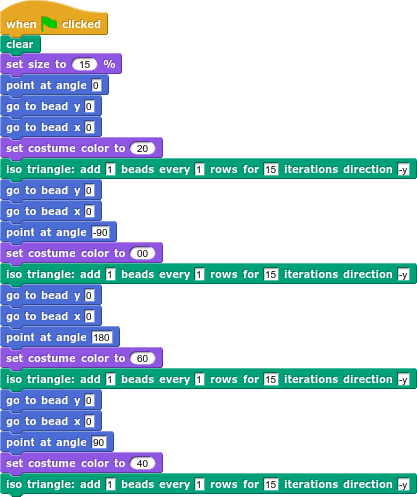
\includegraphics{sample_csnap_applications/alpha.png}
\end{figure}

\begin{figure}[h]
	\caption{Sample Project Beta}
	\label{beta}
	\centering
	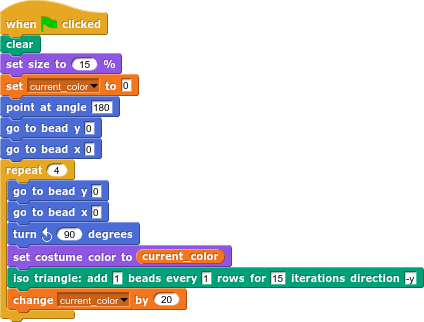
\includegraphics{sample_csnap_applications/beta.png}
\end{figure}

\begin{figure}[h]
	\caption{Sample Project Bravo}
	\label{bravo}
	\centering
	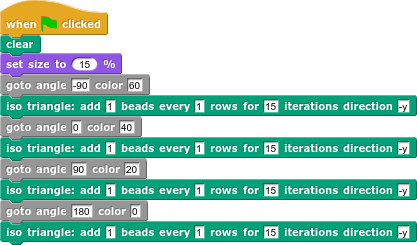
\includegraphics{sample_csnap_applications/bravo.png}
\end{figure}

\begin{figure}[h]
	\caption{Sample Project Charlie}
	\label{charlie}
	\centering
	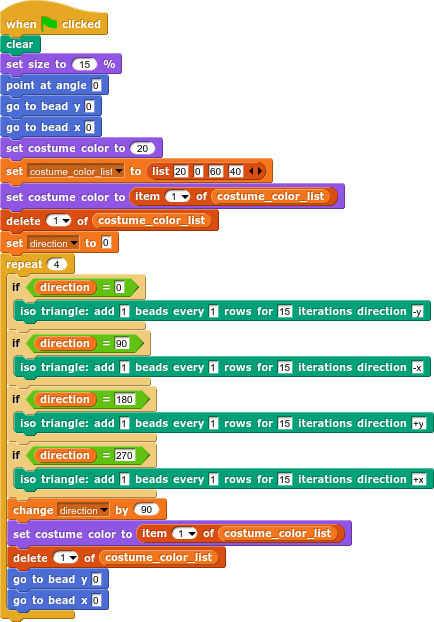
\includegraphics[width=0.75\textwidth]{sample_csnap_applications/charlie.png}
\end{figure}

\begin{figure}[h]
	\caption{Sample Project Delta}
	\label{delta}
	\centering
	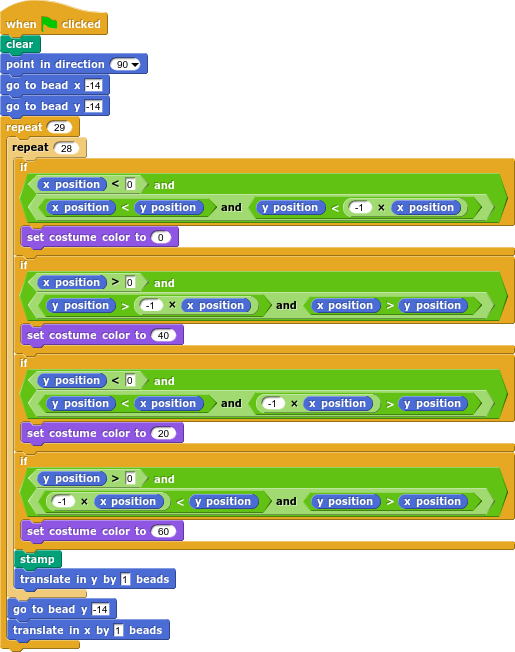
\includegraphics[width=1.0\textwidth]{sample_csnap_applications/delta.png}
\end{figure}

% Repeat with other groups; programmers, crowd sourcing

%% Moorthy
%% Please add papers in bibtex format
%%

\printbibliography

\end{document}
